\documentclass[aspectratio=169]{beamer}%设置宽高比为16:9
\usepackage{graphicx} % 允许包含图像
\usepackage{booktabs} % 允许在表中使用\toprule、\ midrule和\ bottomrule
\usepackage{amsmath}
\usepackage{physics}
\usepackage[]{subcaption}
\usepackage[]{wrapfig}
\usepackage{tikz}
\usepackage{tikzducks}
\usetheme{Darmstadt}
\usecolortheme{default}

\title{Physics on the Celestial}
\author[Author names]{%
		\textbf{Author: } 
		Bufan Zheng\\
		\textbf{Advisor: } 
		Yijian Du
}

\institute[WHU] % 您的机构将出现在每张幻灯片的底部,可能是节省空间的简写
{
	Wuhan University\\ % 你所在的机构
	\medskip
	\textit{whuzbf@qq.com} % Your email address
}
\date{\today} % 日期,可以更改为自定义日期
\begin{document}
	\begin{frame}
		\titlepage % 将标题页打印为第一张幻灯片
	\end{frame}
	
	\begin{frame}
		\frametitle{Overview} % 目录幻灯片
		\tableofcontents 
	\end{frame}
	\section{Lorentz Group}
	\begin{frame}
		\frametitle{Lorentz Group \& Poincar\'e group}
		\begin{definition}
			Lorentz group (O(1,3)) is the isometric transformations in Minkowski spacetime
		\end{definition}
		Four disconnected parts:
		\begin{itemize}
			\item Proper orthochronous lorentz group: $SO(1,3)^\uparrow$
			\item Discret Transformation: $\mathcal{P,T}$
		\end{itemize}
		We just need to care about $SO(1,3)^\uparrow$.
		\begin{definition}
			\[\text{Poincar\'e Group} = SO(1,3)^\uparrow\ltimes \mathbb{R}^{1,3}\]
		\end{definition}
		It's the biggest symmetry group of 1+3 spacetime.
	\end{frame}
	\begin{frame}
		\frametitle{Double Cover}
		As we all know:
		\begin{equation}
			SO(3)\cong SU(2)/\mathbb{Z}_2
		\end{equation}
		Similarly:
		\begin{equation}
			SO(3,1)^\uparrow\cong SL(2,\mathbb{C})/\mathbb{Z}_2
		\end{equation}
		More fun with identities:
		\begin{equation}
			SO(2,1)^\uparrow\cong SL(2,\mathbb{R})/\mathbb{Z}_2,\quad SO(5,1)^\uparrow\cong SL(2,\mathbb{H})/\mathbb{Z}_2,\quad 
			SO(9,1)^\uparrow\cong SL(2,\mathbb{O})/\mathbb{Z}_2
		\end{equation}
		Because
		\begin{theorem}[Hurwitz]
			The normed division algebras over $\mathbb{R}$ are precisely $\mathbb{R},\mathbb{C},\mathbb{H}$ and $\mathbb{O}$.
		\end{theorem}
		So we can never find ternary number!
	\end{frame}
	\section{Celestial}
	\begin{frame}
		\frametitle{Penrose Diagrams (Mink$_4$)}
		Penrose diagram conformally conpactify the spacetime, represent it by a finite scale diagram.
		\begin{figure}
			\centering
		\begin{subfigure}{.4\linewidth}
			\parbox[][6cm][c]{\linewidth}{% 手工指定高度、内容对齐
				\centering
				\includegraphics[width=.6\linewidth]{./figs/2.pdf}}
		\end{subfigure}
		\begin{subfigure}{.4\linewidth}
			\parbox[][6cm][c]{\linewidth}{% 手工指定高度、内容对齐
				\centering
				\includegraphics[width=.8\linewidth]{./figs/1.pdf}}
		\end{subfigure}
		\end{figure}
	\end{frame}
	\begin{frame}
		\begin{definition}
			Every point of $\mathcal{I}^{\pm}$ represent a sphere of infinite radius, called \textbf{Celestial Sphere} ($\mathcal{CS}^2$)
		\end{definition}
		\begin{itemize}
		\item Because $\mathcal{CS}^2$ can be seen as a complex plane after single-point compecting, we can use $(z,\bar z)$ to label its angular coordinates ($\mathcal{S}^2\cong\mathbb{C}\cup \{\infty\}$). We prefer to use retarded coordinates $(u,r,z,\bar z)$ parametrize $\mathcal{I}^+$, and advanced coordinates $(v,r,z,\bar z)$ on $\mathcal{I}^-$. Remember, The angle parameters $(z,\bar z)$ are antipodally identity between $\mathcal{I}^\pm$.
		\item $SO(1,3)^\uparrow\cong SL(2,\mathbb{C})/\mathbb{Z}_2$, Lorentz transformations generate conformal transformations on the celestial sphere!
		\begin{equation}
			z\mapsto \frac{az+b}{cz+d},\quad \bar z\mapsto \frac{\bar a\bar z+\bar b}{\bar c\bar z+\bar d}
		\end{equation}
		\end{itemize}
		We can use infinite symmetry on CFT$_2$ to analyse scattering process in Mink$_4$
	\end{frame}
	\begin{frame}
		\frametitle{Conformal Basis}
		In QFT, we usually use fourier transformation to work in moment space, which can manifest the translational symmetry of Mink$_{d}$. To use the conformal symmerty of CFT$_{d-2}$, we can work with \textbf{Conformal Basis}:
		\begin{itemize}
			\item Photons:
			\begin{equation}
				A_{\mu a}^{\Delta,\pm}(X^{\mu};\vec{w})=-\frac1{(-q\cdot X\mp i\epsilon)^{\Delta-1}}\frac\partial{\partial X^{\mu}}\frac\partial{\partial w^a}\log(-q\cdot X\mp i\epsilon)
			\end{equation}
			\item Gravitons:
			\begin{equation}
				h_{\mu_1\mu_2;a_1a_2}^{\Delta,\pm}(X;\vec{w})=P_{a_{1}a_{2}}^{b_{1}b_{2}}\frac{1}{(-q\cdot X\mp i\epsilon)^{\Delta-2}}\partial_{b_{1}}\partial_{\mu_{1}}\log(-q\cdot X\mp i\epsilon)\partial_{b_{2}}\partial_{\mu_{2}}\log(-q\cdot X\mp i\epsilon)
			\end{equation}
			where $P_{a_1a_2}^{b_1b_2}\equiv\delta_{(a_1}^{b_1}\delta_{a_2)}^{b_2}-\frac{1}{d}\delta_{a_1a_2}\delta^{b_1b_2}$, $\Delta\in\frac d2+\text{i}\mathbb{R}$.
		\end{itemize}
		However, in the soft region, which forced $\Delta=1$, the conformal wave functions need to be redefined. (arXiv: 1810.05219)
	\end{frame}
	\begin{frame}
		For example, we can use Mellin transformation to transform momentum space amplitudes to conformal space amplitudes:
		\begin{equation}
			\widetilde{\mathcal{A}}(\Delta_i,\vec{w}_i)\equiv\prod_{k=1}^n\int_{\mathrm{H}_{d+1}}[d\hat{p}_k]G_{\Delta_k}(\hat{p}_k;\vec{w}_k)\mathcal{A}(\pm m_i\hat{p}_i^\mu)
		\end{equation}
		3 massive scalar scattering ($\phi^3$\mbox{-}theory) at tree-level ($m_\mathrm{in}=(2+\epsilon)m_\mathrm{out}$):
		\begin{equation}
			\widetilde{\mathcal{A}}=\frac{i2^{\frac92}\pi^6\lambda\Gamma(\frac{\Delta_1+\Delta_2+\Delta_3-2}{2})\Gamma(\frac{\Delta_1+\Delta_2-\Delta_3}{2})\Gamma(\frac{\Delta_1-\Delta_2+\Delta_3}{2})\Gamma(\frac{\Delta_1-\Delta_2+\Delta_3}{2})\Gamma(\frac{-\Delta_1+\Delta_2+\Delta_3}{2})\sqrt{\varepsilon}}{m^4\Gamma(\Delta_1)\Gamma(\Delta_2)\Gamma(s_3)|w_1-w_2|^{\Delta_1+\Delta_2-\Delta_3}|w_2-w_3|^{\Delta_2+\Delta_3-\Delta_1}|w_3-w_1|^{\Delta_3+\Delta_1-\Delta_2}}+\mathcal{O}
		\end{equation}
		But we need a more systematic approach, CCFT is comming!
	\end{frame}
	\section{Strominger's Infrared Triangle}
	\begin{frame}
		\frametitle{Infrared Triangle}
		Surprisingly, three seemingly unrelated areas can be linked by some kind of relationship!
		\begin{figure}
			\centering
			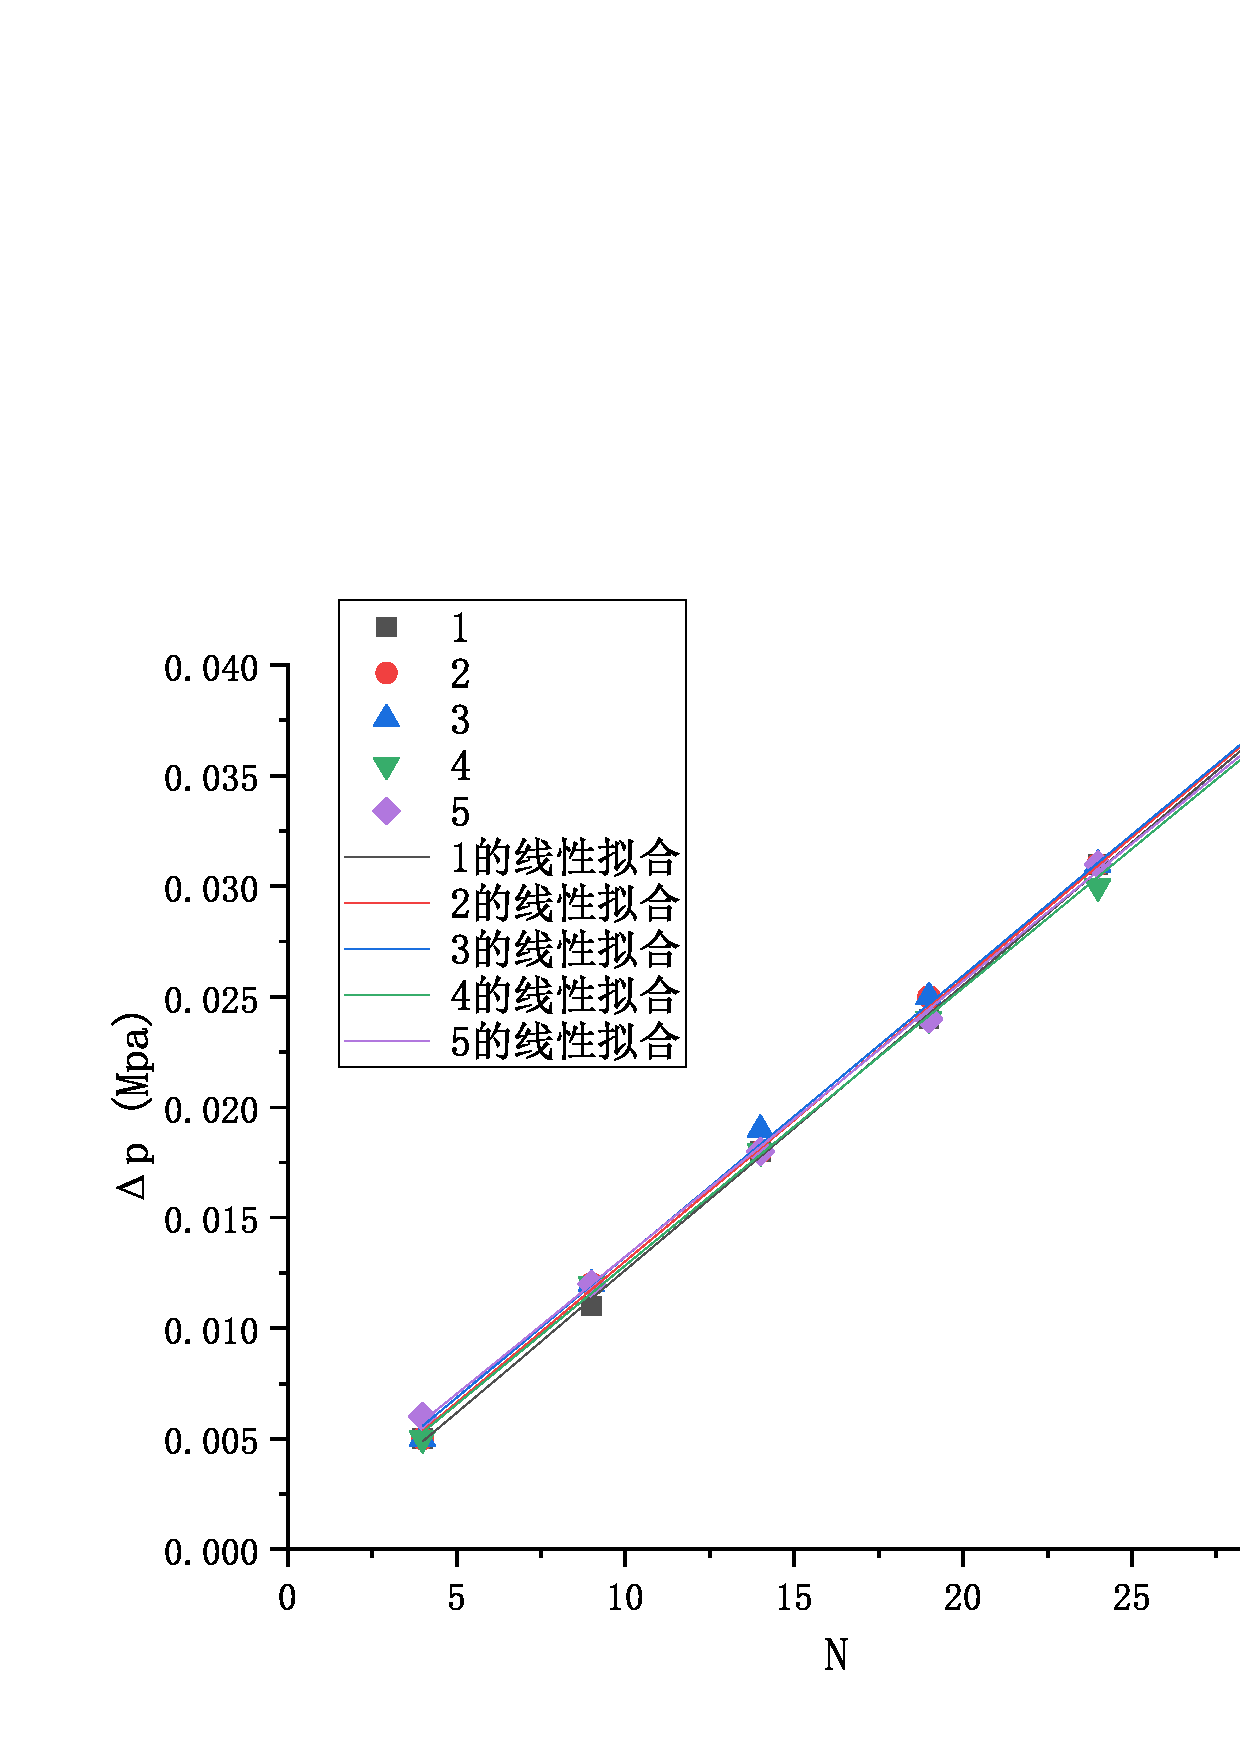
\includegraphics{./figs/3.pdf}
			\caption{The infrared triangle}
		\end{figure}
	\end{frame}
	\begin{frame}
		\frametitle{Large gauge symmetry $\nsubseteq$ Gauge symmetry}
		\begin{definition}
			\[\text{Asymptotic symmetries}=\frac{\text{Allowed symmetries}}{\text{Trivial symmetries}}\]
		\end{definition}
		
		We can use Asymptotic analyse on QED and perturbative gravity to find asymptotic symmetries, called Large gauge/diffeomorphic symmetry. Noether theorem tells us there must be some conserved charges correspond to asymptotic symmetries, in fact, there are infinite number of conserved charges! These symmetries will spontaneous breaking and bring soft photons and soft gravitons to our world. 
		
		\begin{equation}
			\langle\mathrm{out}|\left(Q_\varepsilon^+\mathcal{S}-\mathcal{S}Q_\varepsilon^-\right)|\mathrm{in}\rangle=0\iff
			\sum_{k=1}^m\frac{eQ_k^\mathrm{out}p_k^\mathrm{out}\cdot\varepsilon}{p_k^\mathrm{out}\cdot q}-\sum_{k=1}^n\frac{eQ_k^\mathrm{in}p_k^\mathrm{in}\cdot\varepsilon}{p_k^\mathrm{in}\cdot q}
		\end{equation}
		Asymptotic symmetries$\overset{\text{Ward Indentity}}{\iff}$Soft theorem!
	\end{frame}
	\section{Open Questions}
	\begin{frame}
		\frametitle{Open Questions}
		There are some open questions:
		\begin{itemize}
			\item CCFT
			\item Non-Abelian promotion
			\item Supersymmetry on the celestial 
			\item BCFW, CHY, KLT relations of the celestial $\mathcal{A}$mplitudes
			\item \ldots
		\end{itemize}
		There's a lot of new physics on the celestial waiting to be discovered !
	\end{frame}
	\begin{frame}
		\begin{figure}
			\centering
			\includegraphics[width=.8\linewidth]{./figs/4.png}
		\end{figure}
		\begin{figure}
			\centering
			\includegraphics[width=.8\linewidth]{./figs/5.png}
		\end{figure}
	\end{frame}
	\section*{Thanks}
	\begin{frame}
		\centering
		
\begin{tikzpicture}[scale=2]
			\duck[harlequin=blue,niuqelrah=red,speech={Thank you!},signpost={100}]
		\end{tikzpicture}
	\end{frame} 
\end{document}